\documentclass[a4paper,12pt,oneside]{book}
\usepackage{algorithm}
\usepackage{algorithmic}
\usepackage{geometry}
\usepackage{fixltx2e}
\usepackage{graphicx}
\usepackage{url}
\usepackage{color}
\usepackage{amsmath}
\usepackage{amsfonts}
\usepackage{amssymb}
\usepackage{subfig}
\usepackage{makeidx}
%\usepackage{wrapfig}
%\usepackage{fullpage}
\usepackage{alltt}
%\usepackage[algoruled]{algorithm2e}
\usepackage{setspace}
\usepackage{listings}
\usepackage{verbatim}
%\usepackage{framed}
%\usepackage{multirow}
\usepackage[bookmarks]{hyperref}
\usepackage{array}
%\usepackage{breqn}
\usepackage{amsthm}
%\usepackage{mathtools}
\usepackage{hyperref}
%\usepackage{capt-of}
\usepackage{multicol}
\usepackage{arydshln}
\usepackage{titlesec}
\usepackage[T1]{fontenc}
\DeclareUnicodeCharacter{0301}{\'{e}}



\setlength{\parindent}{0pt}
\theoremstyle{plain} 
\newtheorem{castheorem}{Theorem}[chapter]

\linespread{1.5}
\setcounter{MaxMatrixCols}{20}
\geometry{tmargin=0.85in,  bmargin=0.85in, lmargin=1.4in,  rmargin=0.8in}
\makeindex
\pagestyle{empty}
\begin{titlepage}
\thispagestyle{empty}
    \title{\bfseries \Large Data Analysis and Optimization of Asset Liability Management Problem for Banks}
  %  \author{A dissertation submitted to the University of Hyderabad\\in partial fulfillment of the degree of \\ \\
  %  \bf \Large{Master of Technology}\\in\\ \bf \Large{Artificial Intelligence}\\ \\ By\\ \bf{Gopal Kalpande}\\ \bf{17MCMI10}\\ \\
  %  {
\includegraphics[width=1.3in]{figures/uohyd.jpg}}
  %  \\School of Computer and Information Sciences
  %  \\University of Hyderabad
  %  \\Prof. C. R. Rao Road, Gachibowli, Hyderabad - 500 046} 
\end{titlepage}

\renewenvironment{frontmatter}{\pagenumbering{roman}}{\newpage
        \pagenumbering{arabic}}
\newenvironment{abstract}{\null\vfil\prefacesection{Abstract}}{\par\vfill\null}
\newenvironment{acknowledgments}{\null\vfil\prefacesection{Acknowledgments}}{\par\vfill\null}
\newenvironment{abbrevations}{\null\vfil\prefacesection{Abbreviations}}{\par\vfill\null}
\newenvironment{notations}{\null\vfil\prefacesection{Notations}}{\par\vfill\null}
\renewcommand{\bibname}{Bibliography}

\newenvironment{dedication}
{ \centering
  \thispagestyle{empty}
  \clearpage\null\vfill
  \sl {\large To,}\\
  \hspace{1.5in}}{
  \vspace{3in}\vfill\null}
  \def\prefacesection#1{
  \chapter*{#1}
  \addcontentsline{toc}{chapter}{#1}
  \markboth{#1}{#1}
}

\date{}
\newcommand\tab[1][1cm]{\hspace*{#1}}
\begin{document}
	\maketitle
	\pagestyle{plain}
	
%------------------------------------------------------------Front Matter--------------------------------------------------------------	
	\begin{frontmatter}
	
		%\newpage
		%{
\thispagestyle{empty}
\begin{center}
{ 
\includegraphics[width=1.5in]{./figures/uohyd.jpg}}

\textbf{\large CERTIFICATE}  
\end{center}
\vspace{.50in}
This is to certify that the dissertation entitled ``\textbf{Data Analysis and Optimization of ALM Problem}'' submitted by \textbf{Gopal Kalpande }, bearing Reg. No. 17MCMI10, 
in partial fulfillment of the requirements for the award of Master of Technology in Artificial Intelligence is a bonafide work carried out by him under my supervision and guidance at the Center for Mobile Banking (CMB), IDRBT during 2018 - 2019. \\

The dissertation has not been submitted previously in part or in full to this or any other University or Institution for the award of any degree or diploma.

\vspace{1in}
\noindent

\mbox
{
\parbox[t]{3in}{
\raggedleft
\flushleft 
Dr. V. N. Sastry\\
Project Supervisor\\
Professor and Head (CMB)\\
IDRBT\\}
\hspace{1.75cm}

\parbox[t]{3in}{
\raggedright
\flushleft
 Prof. K. Narayana Murthy\\
Dean\\
School of CIS\\
University of Hyderabad\\}

}

}
	
		%\newpage
		%\begin{center}
\textbf{\large DECLARATION}
\end{center}
\vspace{.50in}
I, Gopal Kalpande hereby declare that this dissertation entitled 
``\textbf{Data Analysis and Optimization of Asset Liability Management Problem for Banks}'' 
submitted by me under the guidance and supervision of \textbf{Dr. V.N. Sastry} is a bonafide work which is also free from plagiarism. 
I also declare that it has not been submitted previously in part or in full to this University or other University or Institution for the award of any degree or diploma. I hereby agree that my dissertation can be deposited in Shodganga/INFLIBNET.

\vspace{1in}

\noindent
\parbox[t]{3in}
{\raggedright
Date:\\
Place:\\
}
%\nobreak
\parbox[t]{3in}
{
\raggedleft 
(Gopal Kalpande)\\
17MCMI10\\
}
        \vspace*{2.5cm}\centerline{//Countersigned//}

        \noindent%
        Signature of the Supervisor(s):

        \vspace*{1.5cm}\noindent(Dr. V. N. Sastry)
        

	
		%\begin{dedication}
		%	\thispagestyle{empty}
		%	{{\bf My Parents}}
		%\end{dedication}
	
		%\begin{acknowledgments}
		%	I would like to express my sincere gratitude to {\bf Dr. V. N Sastry}, my project supervisor, 
for valuable suggestions and keen interest through out the progress of my course of research. \\

I would like to thank {\bf Prof. N. P. Dhavale} for his valuable suggestions through out the project.\\

I am grateful to the {\b fHead, Center for Mobile Banking} for providing excellent computing facilities 
and a congenial atmosphere for progressing with my project. \\

I would like to thank {\bf Institute fot Development and Research in Banking Technology, Hyderabad} for providing all the necessary resources for the successful completion of my course work. At last, but not the least I thank my classmates and 
other students of SCIS for their physical and moral support. \\

I would also like to thank the {\bf Open Source Community} who provided the free Software and documentation to work with.

\vspace{0.7in}

\begin{flushright}
With Sincere Regards,\\
{\bf Gopal Kalpande}
\end{flushright}


		%\end{acknowledgments}

		%\begin{notations}
		%	{\bf For Deep Learning Concepts:}\\
A: Recurrent layer of neurons\\
w$_{i}$:  weight associated with the inputs in RNN\\
w$_{o}$:  weight associated with the output of previous state in RNN\\
X$_{t}$: input sequence\\
h$_{t}$: output of the t$^{th}$ recurrent layer\\
f$_{t}$: is the output of forget gate\\
i$_{t}$: is the output of input gate\\
W$_{f}$: the weight associated with forget gate\\
W$_{i}$: the weight associated with input gate\\
W$_{o}$: the weight associated with output gate\\
W$_{c}$: the weight associated with new candidate value for input gate\\
$\tilde{I}_{t}$ : vector of new candidate values for input gate\\
h$_{t-1}$: the previous state output\\
C$_{t}$: Cell state\\
o$_{t}$: output of the output gate\\
X$_{t}$: the input to state t\\
b$_{f}$: the bias term for forget get\\
b$_{i}$: the bias term for input get\\
b$_{o}$: the bias term for output get\\
b$_{c}$: the bias term for candidate value for input gate\\
e($\hat{y}_{t-1}$): Encoding of previous states output

terms in []: reflects concatenation operation\\
$\sigma$ : Sigmoid Function\\
tanh : hyperbolic tan function\\

{\bf For LPP Formulation}:\\
G: Gap value\\
Y : Asset\\
X: Liability\\
a: investment time bucket\\
b: maturity time bucket\\
c: Asset/Liability Number\\
c$_{j}$ : (j =1,2,...n) Profit Coefficient \\
b$_{i}$ : (i = 1,2,...m) resource limitation \\
a$_{i,j}$ : (i = 1,2,..m) (j =1,2,...n) input output coefficient \\ 
S$_{i}$ : Slack variable \\ 
B : Basic variable in the basis \\ 
C$_{Bi}$ : Coefficient of current basic variable in objective function \\ 
c$_{j}$ : Coefficient of variables in objective function \\ 
z$_{j}$ : $\sum$ a$_{i,j}$C$_{Bi}$ where i =1,2,...m and j = 1,2,..., n+m \\ 
X$_{B}$ :  Solution Values of basic variables \\ 
c$_{j}$ - z$_{j}$ : Max value of this gives key column. \\ 
Ratio$_{i}$ : Min value of this gives key row, leading to selection of key element \\ 



		%\end{notations}	

		%\begin{abstract}
		%	%\section{Abstract}
Inter dependence of financial market around the globe is well established. The same has opened the banking to various risks. The objective of the project is to ALM in banks and to minimize financial risks. Asset and liability management is an important problem in finance, which mainly focuses on controlling the liquidity risk and interest rate risk.\\

The First chapter of the thesis contains the elaborate view on the risks associated with banking, ALM process as per the guidelines of RBI, project objective, problem statement and the detailed literature survey with background knowledge. The thesis mainly focuses on the simulation of ALM problem for banks which will be discussed in chapter 2, LPP formulation for optimization of assets discussed in chapter 3 and prediction of stock price using LSTM neural network discussed in chapter 4. The chapter 5 contains the conclusion of the thesis and future directions are in chapter 6.

%As part of these projects we expect the students to develop some of the existing schemes and, if possible, to come up with new schemes realizing the compartmented access structures.

		%\end{abstract}
	

		%\tableofcontents

		%\listoffigures

		%\listoftables


		
	%	\notations	
	
	\end{frontmatter}
%--------------------------------------------------------------------------------------------------------------------------------------

%----------------------------------------------------------Main Matter-----------------------------------------------------------------	

	\renewcommand{\baselinestretch}{1.7}
	
	\chapter{Introduction}
	\setcounter{secnumdepth}{4}

\titleformat{\paragraph}
{\normalfont\normalsize\bfseries}{\theparagraph}{1em}{}
\titlespacing*{\paragraph}
{0pt}{3.25ex plus 1ex minus .2ex}{1.5ex plus .2ex}


In this chapter, first, we learn about the risks associated with banking. Then we will discuss Asset Liability Management (ALM) a solution to minimize risk associated with banking. Then we will discuss project objectives and problem statement. Then a glance over banking standards and the literature survey.\cite{}

\section{Risks Associated with Banking}

The term risk can be defined in association with banking as the exposure to loss.  The several risks associated with banking are viz.,
Operational risk, Credit risk, Liquidity risk, Market risk, Foreign exchange risk, Interest rate risk and Information risk.

	\subsection{Operational Risk}

		It is defined as the loss occurred due to failure of peoples or system. It is faced in the various departments as of Information Technology department, Credit Department, Investment department.

	\subsection{Credit Risk}

		It is defined as the loss occurred due to failure of the borrower to repay to bank on the agreed terms. There is uncertainty about the repayment of dues and in the repayment in the agreed time frame. It happens due to borrowers lack of income, failure of business or reluctance to repay and lack of underwriting frameworks.

	\subsection{Market risk}

		It is defined as the loss occurred due to fluctuation in the market prices. Its components are as follows:
		
		\begin{itemize}
		
			\item \textbf{Equity risk: }Probable failure to generate profit due to fluctuation in stock prices.
			
			\item \textbf{Foreign exchange risk: }Probable failure to generate profit due to the fluctuation of exchange rates as bank does transaction in multiple currencies.
			
			\item \textbf{Interest rate risk: }Probable failure to generate profit due to the fluctuation of interest rates.
			
			\item \textbf{Commodity risk: }Probable failure to generate profit due to change in commodity prices as metals (as gold, silver, platinum), Energy (oil and gas) and Agriculture (as wheat, cotton, coffee, tea,etc.). The change in these prices occurs due to variations in demand and supply.

		\end{itemize}

	\subsection{Liquidity risk}

		It is characterized as the lack of liquid cash available in hands of the bank to finance its day to day transactions or the situation where bank runs out of cash. Failure in managing the liquidity risk can lead to the destruction of the banks' reputation and losing its trust among customers.

The exposure of banks to these various risks and as the risks are also increasing with the liberalisation and increasing merger of local markets and global markets. Due to the deregulated operational space and the various products that requires the interest rates to be determined with the need to maintain the proper ratios between the profitability, spread and long term growth. Due to all these reasons, we need to perform Asset Liability management.


	
\section{Asset Liability Management (ALM)}

	An asset is a valuable entity/resource that a person/organization owns for generating income.  And the liability is a valuable entity/resource that a person/organization needs to pay for. At any given point of time, total assets must be greater than the total liability. To balance the equation the concept of asset liability management \cite{11} had emerged. 

	In ALM we perform periodic monitoring of risk exposures involving collecting and analyzing the information in order to have the ability to anticipate, forecast and act so as to structure banks business to profit. ALM also involves transforming the asset and liability portfolio in a dynamic way to manage the risks which involve judgment and decision making.

%ALM involves the planning, directing and controlling the cash flow and yield of the consolidated funds of the bank for all %assets and liabilities of a bank by rate, amount and maturity. It assesses the various asset mixes, funding combinations, %price volume relations and their implications on liquidity, income and capital ratio.


	
\section{ALM for Banks}

	As the business of banking involves lot of risks, the main problem of banking becomes risk management and the procedure to do so is ALM. The three pillars on which ALM resides are follows:

	\subsection{ALM Information System}
		The risk policies and tolerance limits need to be specified by ALM information system. Information is the key to ALM process which is now available due to the computerization of all banks and its respective branches. It also includes performing experimentation in a specific branch and studying its effects. If the results are positive then replicating the changes to other branches.

	\subsection{ALM Organization}
		For risk management to be successful the need is strong commitment of the senior management to take strategic decisions and integrate the basic operations. The Asset Liability Committee (ALCO) is formed for performing the above-mentioned tasks. It includes the CEO and the senior management of the bank, and their task is to decide business strategies with respect to banks budget and decide risk management objectives according to assets and liabilities. 

	\subsection{ALM Processes}
		The ALM Processes are as shown in the following figure:
		
		\begin{center}
		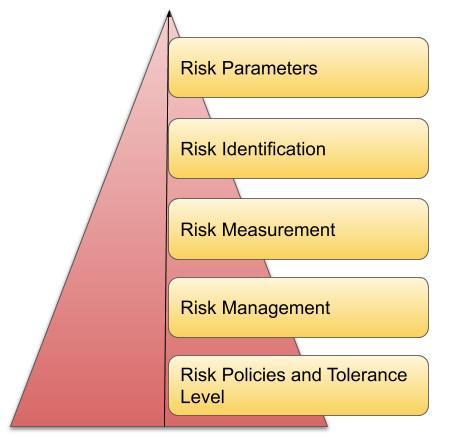
\includegraphics[width=\linewidth]{figures/ALM_Process.jpg}	
		\captionof{figure}{ALM Processes}
		\label{fig:ALM Processes}
		\end{center}
		

		All the risks discussed in section 1.1 are the problems to be handled by the ALM Processes. The assets and liabilities of a bank involve the following:

		\begin{center}
		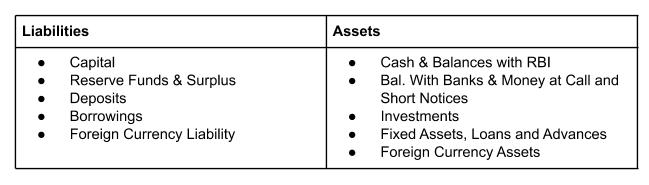
\includegraphics[width=\linewidth]{figures/Components_of_Banks_Balance_Sheet.jpg}	
		\captionof{figure}{Components of Banks Balance Sheet}
		\label{fig:Components of Banks Balance Sheet}
		\end{center}
	
		The ALM cycle of a bank is as follows:

		\begin{center}
		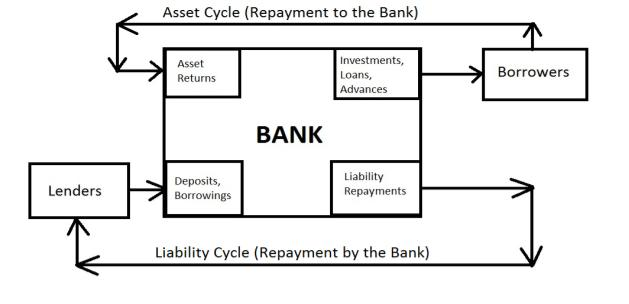
\includegraphics[width=\linewidth]{figures/ALM_Cycle_of_a_Bank.jpg}	
		\captionof{figure}{ALM Cycle of a Bank}
		\label{fig:ALM Cycle of a Bank}
		\end{center}

		Throughout the cycle of the ALM the mismatch in asset and liabilities (negative gap) should not exceed 20\% of the cash outflow during 2-14 days and 15-28 days time bucket.

	
\section{Project Objective}

	To study the strategies to stabilize financial networks i.e. banks and to improve the profitability of them from various risks. 

\section{Problem Statement}

	The two problems that have been studied are as follows:
	\subsection{Liquidity Risk Management}

Simulation of the ALM concept for bank using the 1999 Czech Financial data set and try the single objective cash flow optimization for ALM to ensures Liquidity and Profitability of the bank. 

	\subsection{Prediction of Stock Price}

		The Prediction of Stock Price is a typical problem of time series and we use a deep learning based solution for future price prediction.

\section{Literature Survey}

	For first problem the literature survey done is: Hongxi Li et al. (2017) assess for both positive and negative duration gap to increase the net value of bank when interest rates fluctuate favorably\cite{4}. Nalan Gülpinar et al. (2013) uses the Vector Autoregressive process to model time-varying investment opportunities\cite{3}. Teng Fan et al. (2011) studied the interest rate risk of Chinese life insurers’ liability\cite{1}. Mounika, P et al. (2011) have addressed the problem of single objective optimization for the maximization of wealth\cite{16}. Chaudhury, Rahul et al. (2014) created a fuzzy rule-based asset liability optimization model\cite{17}.

	For the second problem, the literature survey done is: Ashish Vaswani et al. (2017) proposed an attention mechanism for machine translation\cite{2}. Yao Qin et al. (2017) proposed a DA-RNN. It serves the purpose of attention to time series and encoding information of long sequences\cite{6}. Jian Liu et al. (2017) assesses the correlation between stock price movement with relevance to events happening in the world\cite{7}. Hao Li et al. (2018) proposed the MI-LSTM using attention which filters noise and extracts information\cite{8}. Huicheng Liu (2018) used attention based RNN for leveraging the news to predict stock price\cite{9}.

Below are the existing algorithms which helps as basis for problems we are studying. The implementation of some of these methods is available in a software package called \emph{statsmodels, pandas, sklearn} \cite{5} \cite{12}, which are also necessary statistical analysis.


%--------------------------------------------------------------------------------------------------------------------------------------

\subsection{Time Series Analysis for Stock Price Prediction}

	\subsubsection{Introduction}
		The Time Series (TS) is defined as the collection of information or data at a regular interval of time. This TS contains the time-dependent data which may contain the seasonality (i.e the deviation in data at specific time frame) and trend (i.e. the changing mean with respect to time) in it; which is the change in data with respect to specific time frame.

		Ex. The Stock Data is collected per day i.e. the value of stock at the start of the day, at the end of the day, the highest value of the day and the lowest value of the day.

		\begin{center}
		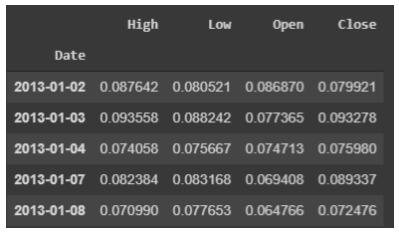
\includegraphics[width=\linewidth]{figures/Ex_of_Time_Series_data_of_a_stock.jpg}	
		\captionof{figure}{Ex of Time Series data of a stock}
		\label{fig: Ex of Time Series data of a stock}
		\end{center}


	
	\subsubsection{Issues with non-Stationarity of Data}
	
		The data is said to be stationary if the mean and variance of the data is stable over time and it has time-independent autocovariance. The statistical models which deal with the TS data have a premise that the data should be stationary. Because of this premise, we need to convert non-stationary data to stationary data. But how to check the data is stationary or not? There are two ways to do it:
		\begin{itemize}
		
			\item Plotting the Rolling Statistics
			
			\item Dickey-Fuller Test

		\end{itemize}
		
		\paragraph{Plotting the Rolling Statistics}

			In this procedure, we visualize the moving average and/or moving variance by plotting it against time.

		\begin{center}
		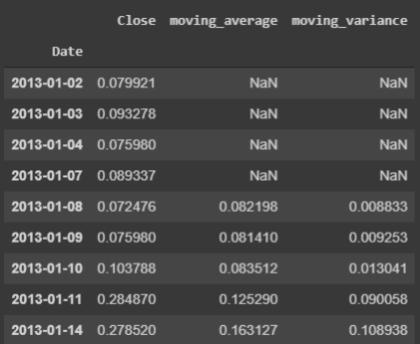
\includegraphics[width=\linewidth]{figures/Moving-Average-and-Moving-Variance.jpg}	
		\captionof{figure}{ Moving Average and Moving Variance of the Closing Price with window size = 5}
		\label{fig: Moving Average and Moving Variance of the Closing Price with window size = 5}
		\end{center}

		\begin{center}
		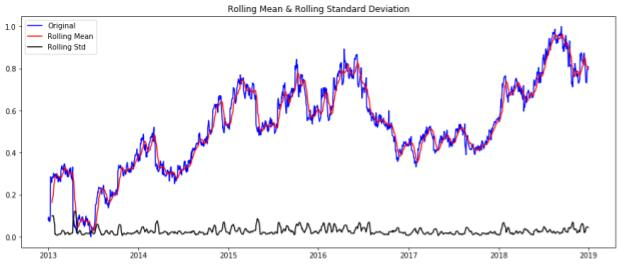
\includegraphics[width=\linewidth]{figures/Plot-of-the-Rolling-Mean-and-the-Rolling-Standard-Deviation.jpg}	
		\captionof{figure}{Plot of the Rolling Mean and the Rolling Standard Deviation of Moving Average of Closing Price}
		\label{fig: Plot of the Rolling Mean and the Rolling Standard Deviation of Moving Average of Closing Price}
		\end{center}
	
			As we can infer from the plot, the rolling mean is changing with respect to time and there is a clear fluctuation in the standard deviation resulting in the data to be non-Stationary.

		\paragraph{Dickey-Fuller Test (DF Test)}

		In statistics, there is a unit root test that is used to check the given TS is non-Stationary or not. DF Test \cite{18} is the most widely used unit root test. In statistical testing we have to make the hypothesis, the same in this test are:

H0:	TS is non-Stationary.
H1:	TS is Stationary.

H0 is the Null hypothesis and the H1 is the Alternate Hypothesis. The hypothesis H0 is accepted if the p-value of the test is greater than 5\% else the H0 is rejected and H1 is accepted.

For the data we are dealing with the results of the DF Test are as follows:

		\begin{center}
		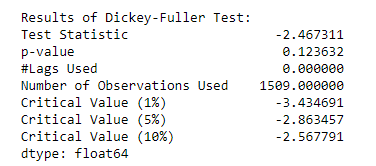
\includegraphics[width=\linewidth]{figures/DF-Test-Results-for-moving-average-of-Closing-price.jpg}	
		\captionof{figure}{DF Test Results for moving average of Closing price}
		\label{fig: DF Test Results for moving average of Closing price}
		\end{center}
	
		As the p-value is 0.1236 i.e. 12.36\% which is greater than the threshold 5\% so the null hypothesis H0 is accepted; meaning the TS is non-Stationary.

	\subsubsection{Converting non-Stationary TS to Stationary TS}
	
		To make the TS stationary we need to eliminate the trend and seasonality from the non-stationary TS. The first and the widely used approach to do it is Transforming the data using a log transform. Then use either Differencing or Decomposition. Let’s see them one by one:

		\paragraph{Log Transform}
			Taking the log of the data changes the recurrent pattern to a linear pattern and also stabilizes the variance of the data \cite{18}.

		\begin{center}
		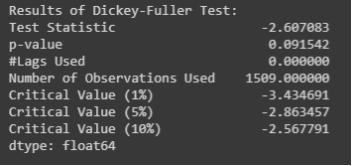
\includegraphics[width=\linewidth]{figures/DF-Test-Results-for-log-transformed-Closing-price.jpg}	
		\captionof{figure}{DF Test Results for log-transformed Closing Price}
		\label{fig: DF Test Results for log-transformed Closing Price}
		\end{center}

			Here we can see that the p-value is dropped from 12.36\% to 9.15\% which means that we can say we have 90\% confidence that the TS is stationary.

		\paragraph{Decomposing}

			A TS consists of three components: trend, seasonality and residual. If the decomposition be additive then:
				\begin{equation}
					Data\textsubscript{t} = Trend\textsubscript{t} + Seasonality\textsubscript{t} + Residual\textsubscript{t}  
				\end{equation}
				


			Where the subscript t denotes the time t.
			The multiplicative decomposition is:
				\begin{equation}
					Data\textsubscript{t} = Trend\textsubscript{t} * Seasonality\textsubscript{t} * Residual\textsubscript{t} 
				\end{equation}
				

			The addition/multiplication of these three components gives back the original data or TS. The multiplicative decomposition is used when the trend/seasonality of data is proportional to the time.
			The procedure of classical multiplicative decomposition \cite{18} is as follows:

				\begin{algorithm}[H]
					\caption{Classical Multiplicative Decomposition}
					Assumption m - seasional period or frequency, 
	        						MA - moving average, 
	       						DT\textsubscript{t} - Detrended series.

					\begin{algorithmic}[1] 
						\STATE If m is even number then \begin{equation}Trend_{t} = 2 * m-MA		\end{equation}

								Else \begin{equation}Trend_{t} = m-MA	\end{equation}
						\STATE Compute Detrended series:
									\begin{equation}DT\textsubscript{t} = Data\textsubscript{t} - Trend\textsubscript{t} \end{equation}
						\STATE The seasonal component Seasonalitytof the respective season is the average of the DT\textsubscript{t} of the given season.
						\STATE \begin{equation}Residual\textsubscript{t} = Data\textsubscript{t} / (Trend\textsubscript{t}  * Seasonality\textsubscript{t})	\end{equation}
					\end{algorithmic}
				\end{algorithm}

			The plot looks as follows:
				
				\begin{center}
				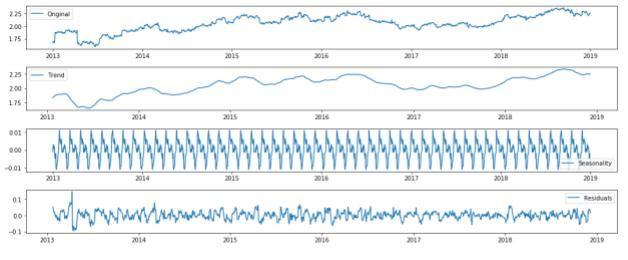
\includegraphics[width=\linewidth]{figures/The-trend-seasonality-and-residual-of-log-transformed-data.jpg}	
				\captionof{figure}{The trend, seasonality and residual of log-transformed data}
				\label{fig: The trend, seasonality and residual of log-transformed data}
				\end{center}

			The result of DF test results on the residual data is as follows:

				\begin{center}
				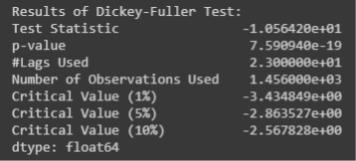
\includegraphics[width=\linewidth]{figures/DF-Test-Results-on-residual-data.jpg}	
				\captionof{figure}{DF Test Results on residual data}
				\label{fig: DF Test Results on residual data}
				\end{center}

			Here the p-value is 7.5e-17\% which means that we can say the TS is stationary with 99.99\% confidence.

		\paragraph{Differencing}

			In this approach, we compute the difference between the data point at the current instance to the previous instance. Applying the DF test on the differencing \cite{18} of the log-transformed data gives the following results:

				\begin{center}
				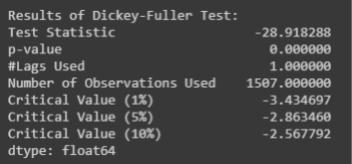
\includegraphics[width=\linewidth]{figures/DF-Test-Results-for-log-transformed-Closing-price-after-differencing.jpg}	
				\captionof{figure}{DF Test Results for log-transformed Closing price after differencing}
				\label{fig: DF Test Results for log-transformed Closing price after differencing}
				\end{center}

			Here the p-value is 0.0\% which means that we can say the TS is stationary with 100\% confidence.


	\subsubsection{Disadvantages of Making TS stationary}

		There is huge information loss when we are converting the non-stationary TS to Stationary TS. The elimination of trend and seasonality leads to information loss which makes the model linear and it fails to predict the future trend and seasonality appropriately. 

	\subsubsection{Inference}

		The statistical methods are good to work with the stationary data, but when the data is non-stationary the statistical methods fail due to the premise discussed in section 3.2. Although due to the advances in the research area of neural networks we are able to deal with the non-stationary data without converting it to stationary. The methods used to predict the TS data are discussed in following section.


\subsection{Deep Learning Architectures for Prediction of Stock Price}

In this chapter, we will study the different deep learning techniques used to predict the sequence of output after feeding them the time-based input sequence. 

For all the tasks consider
Data: {X\textsubscript{i} : Source\textsubscript{i} ; Y\textsubscript{i} : Target\textsubscript{i} }
And the loss function: Mean Squared Error Loss as the problem is a regression problem. 

\subsubsection{Recurrent Neural Network (RNN)}

Artificial neural networks have a special class of neural networks that works best with the input sequences, called the RNN. As stated in the name the word Recurrent stands for the repeating structure of the neurons with respect to time/sequence based input to them until the whole input sequence is over. Unlike other neural network architectures where we need to feed whole input at once to the input neurons; in RNN \cite{12}, we can feed the sequence one by one to the input neurons and the input gets processed in the same recurrent fashion throughout all the recurrent layers. The output of the neuron after processing the (t-1)$^{th}$ input sequence is fed again to the same neuron with the (t)$^{th}$ sequence of the input so that it can remember the whole input sequence. The idea basically is to remember the past, add it to the present and predict the future. The RNN looks as shown in the following Fig.

				\begin{center}
				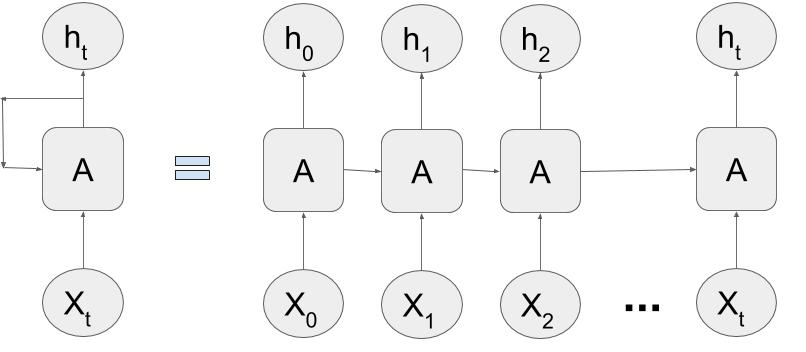
\includegraphics[width=\linewidth]{figures/An-unrolled-recurrent-neural-network.jpg}	
				\captionof{figure}{Unfolded Recurrent layer}
				\label{fig: Unfolded Recurrent layer}
				\end{center}


Now let’s consider the Fig.4.3 which shows the activation function tanh in the neurons of recurrent layers. The equation of the recurrent layer is as follows:

\begin{equation}
	h_{t} = tanh (w_{i} * X_{t} + w_{o} * h_{t-1} + b)
\end{equation}


Where wi is the weight associated with the inputs and the wo is the weights associated with the output of the previous state. Using these weights we will learn about the sequenced input.

				\begin{center}
				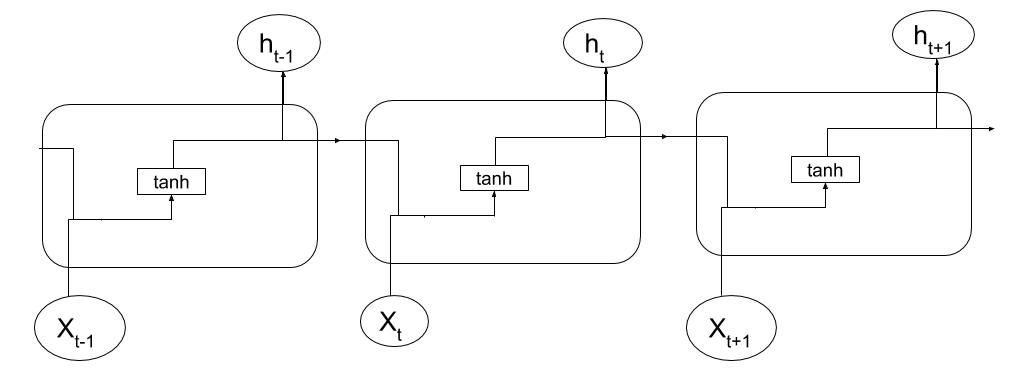
\includegraphics[width=\linewidth]{figures/The-repeating-module-in-a-standard-RNN.jpg}	
				\captionof{figure}{Unfolded Recurrent layer with activation function}
				\label{fig: Unfolded Recurrent layer with activation function}
				\end{center}


\paragraph{Problems of Long Term Dependency}

If the input sequences are small then the RNN is the best choice, but what if the input sequence is long, can RNN successfully learn the information from the past and using present information predict the future? The answer is No. In RNN we don’t have an equation for how much to remember from the past or what to remember from the past. This is called the problem of long term dependency \cite{12} as shown in Fig.4.4. If the output ht+1 depends on the input X1 then RNN can’t handle this dependency. The solution to this is the improved version of RNN discussed later.

				\begin{center}
				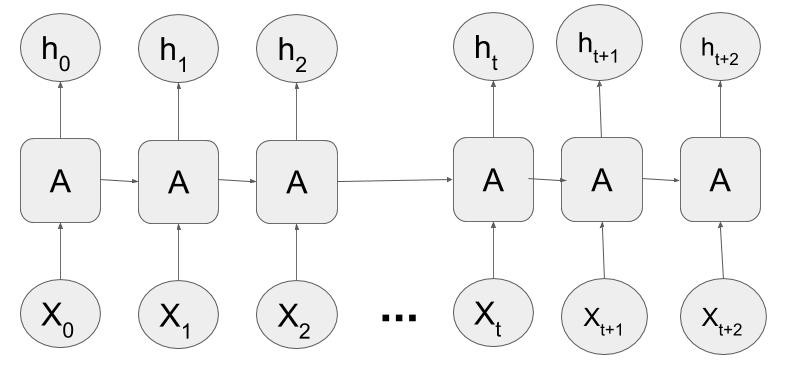
\includegraphics[width=\linewidth]{figures/Problem-of-Long-Term-Dependency.jpg}	
				\captionof{figure}{Long term dependency problem}
				\label{fig: Long term dependency problem}
				\end{center}



\paragraph{Long Short Term Memory (LSTM)}

The word LSTM \cite{12} can be interpreted as storing the Short information in the Memory for the Long Term. This happens due to the functional change in the cell of RNN. Instead of the single neuron function in the RNN, the LSTM has four neurons connected in a circuit creating three gates: input gate, forget gate and the output gate. Other than these gates there is a cell state which computes the update for the next state. The following are the notations that will be used to describe the architecture of the LSTM:

				\begin{center}
				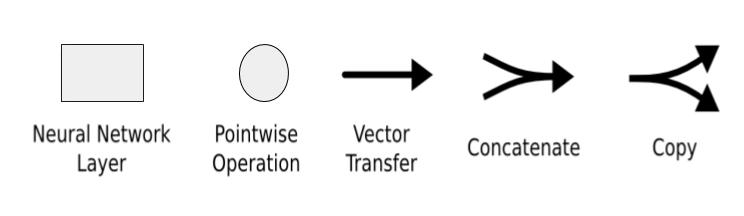
\includegraphics[width=\linewidth]{figures/Notations.jpg}	
				\captionof{figure}{Notations}
				\label{fig: Notations}
				\end{center}

The comparison of RNN and LSTM is as follows:

				\begin{center}
				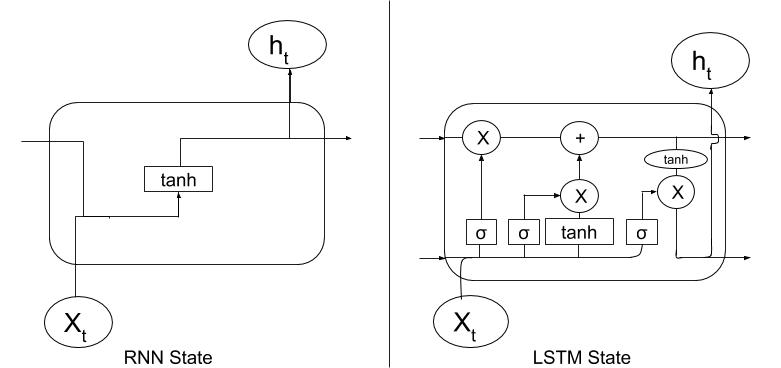
\includegraphics[width=\linewidth]{figures/Comparison-of-RNN-and-LSTM-Cells.jpg}	
				\captionof{figure}{Comparison of RNN and LSTM State}
				\label{fig: Comparison of RNN and LSTM State}
				\end{center}

\subparagraph{Cell State}

The cell state decides how much of the original information from previous state is to be retained to the next state (Forget gate) and how much new information from the current state is to be added after forgetting the old information from the previous state (Input gate). It's like scaling and shifting operation. The information from the previous state is scaled between 0 to 1 and information from the current state is added (shifting).

				\begin{center}
				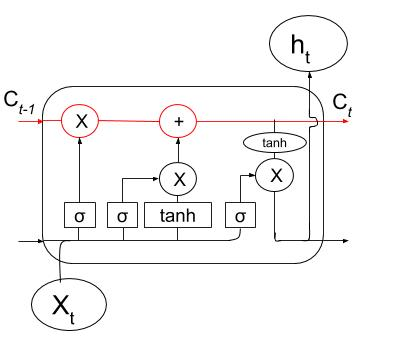
\includegraphics[width=\linewidth]{figures/Cell-State.jpg}	
				\captionof{figure}{Cell State}
				\label{fig: Cell State}
				\end{center}

\subparagraph{Forget Gate}

As discussed in the cell state this gate uses the sigmoid function which gives the values between 0 to 1. These values determine the scaling of the forget gate.
Equation for forget gate:

\begin{equation}
	f_{t} = \sigma (W_{f} . [h_{t-1}, X_{t}] + b_{f})	
\end{equation}

				\begin{center}
				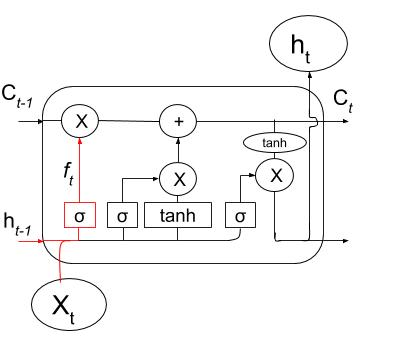
\includegraphics[width=\linewidth]{figures/Forget-gate.jpg}	
				\captionof{figure}{Forget Gate}
				\label{fig: Forget Gate}
				\end{center}

\subparagraph{Input Gate}

This gate decides how much information from the current state is to be added to the cell state. It uses a sigmoid and a tanh function for this purpose. The equation is as follows:

\begin{equation}
	i_{t} = \sigma (W_{i} . [h_{t-1}, X_{t}] + b_{i})
\end{equation}

\begin{equation}
	\tilde{I}_{t} = tanh (W_{c} . [h_{t-1}, X_{t}] + b_{c})	
\end{equation}


The sigmoid function ranges between 0 to 1 and tanh function ranges between -1 to 1 which shifts the input accurately and creates the output of the input gate.

				\begin{center}
				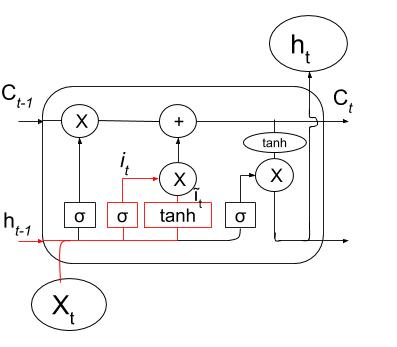
\includegraphics[width=\linewidth]{figures/Input-gate.jpg}	
				\captionof{figure}{Input Gate}
				\label{fig: Input Gate}
				\end{center}

\subparagraph{Updating Cell State}

The eq(2.8 to 2.10) computed the values for updating the cell state, now we just need to do pointwise multiplication and addition. The equation is as follows:

\begin{equation}
		C_{t} = f_{t} * C_{t-1} + i_{t} * \tilde{I}_{t}
\end{equation}

				\begin{center}
				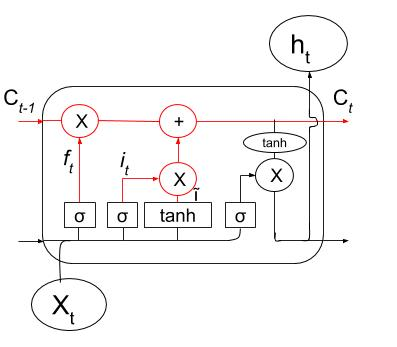
\includegraphics[width=\linewidth]{figures/update-to-new-cell-state.jpg}	
				\captionof{figure}{Update to new cell state}
				\label{fig: Update to new cell state}
				\end{center}


\subparagraph{Output Gate}

Using sigmoid function on current states input and tanh function on the updated cell state we can output the parts we need. The equations are as follows:

\begin{equation}
	o_{t} = \sigma (W_{o} . [h_{t-1}, X_{t}] + b_{o})
\end{equation}

\begin{equation}
	h_{t}  = o_{t} * tanh( C_{t} )
\end{equation}

				\begin{center}
				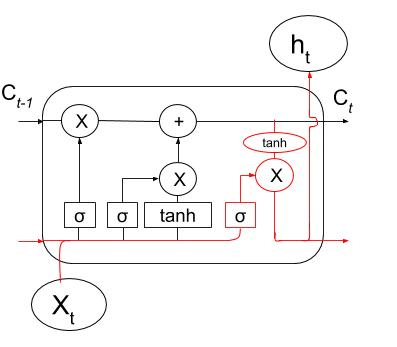
\includegraphics[width=\linewidth]{figures/output-gate.jpg}	
				\captionof{figure}{Output Gate}
				\label{fig: Output Gate}
				\end{center}

The Fig. below shows the unfolded LSTM layer.

For the understanding of the later equations let us consider the following equations:
For RNN: \begin{equation} h_{t} = RNN(h_{t-1}, X_{t}) \end{equation}

For LSTM: \begin{equation} h_{t}, C_{t} = LSTM(h_{t-1}, C_{t-1}, X_{t}) \end{equation} 

\paragraph{Encoder - Decoder Models (Sequence to sequence models)}

The Encoder - Decoder model \cite{12} is very much useful in a lot of applications. The Encoder which is a neural network works for computing the representation of the input while the decoder which is also a neural network uses this input representation from Encoder and the target output to learn about the relation between the input and output and makes the appropriate predictions. For our problem, both encoder and decoder use the RNN/LSTM as the encoding and decoding function. The Encoder - Decoder mechanism can be represented as in Fig. below:

				\begin{center}
				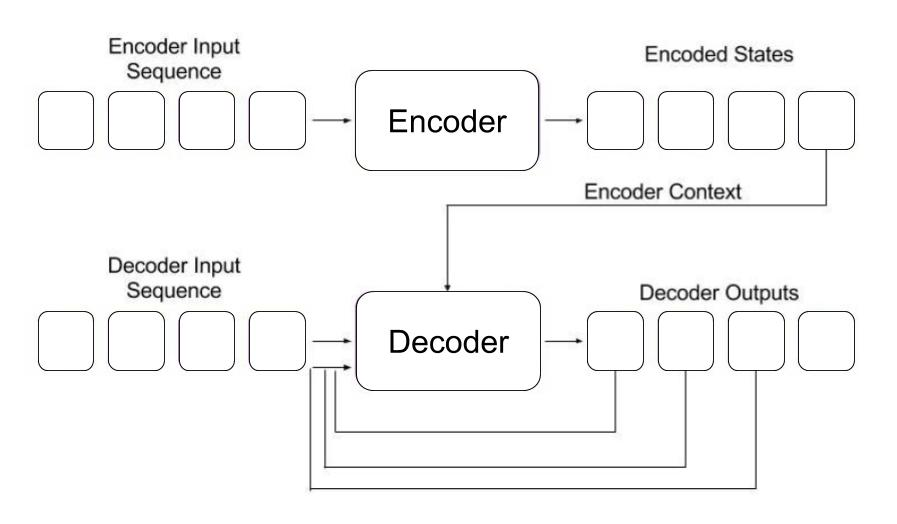
\includegraphics[width=\linewidth]{figures/Sequence-to-Sequence-Model.jpg}	
				\captionof{figure}{Encoder - Decoder Mechanism}
				\label{fig: Encoder - Decoder Mechanism}
				\end{center}

The equations for the encoder-decoder model using RNN as the neural network architecture is as follows:
 
Encoder: \begin{equation} h_{t} = RNN(h_{t-1}, X_{t}) \end{equation}

Decoder: \begin{equation} C_{0} = h_{t}  \end{equation}	
		 \begin{equation} C_{t} = RNN(C_{t-1}, [h_{t-1}, e(\hat{y}_{t-1})])  \end{equation}

%Ct = RNN(Ct-1, [ht-1, e(y_hatt-1)])

\paragraph{Encoder - Decoder Models with attention (Sequence to sequence models with attention)}

The attention is a technique which tells the decoder how much to focus on the information at the given point of time. The attention of the overall input sequence adds to 1 due to the softmax function. The Encoder - Decoder mechanism with attention \cite{2}, \cite{7} can be represented as in Fig.4.13.

				\begin{center}
				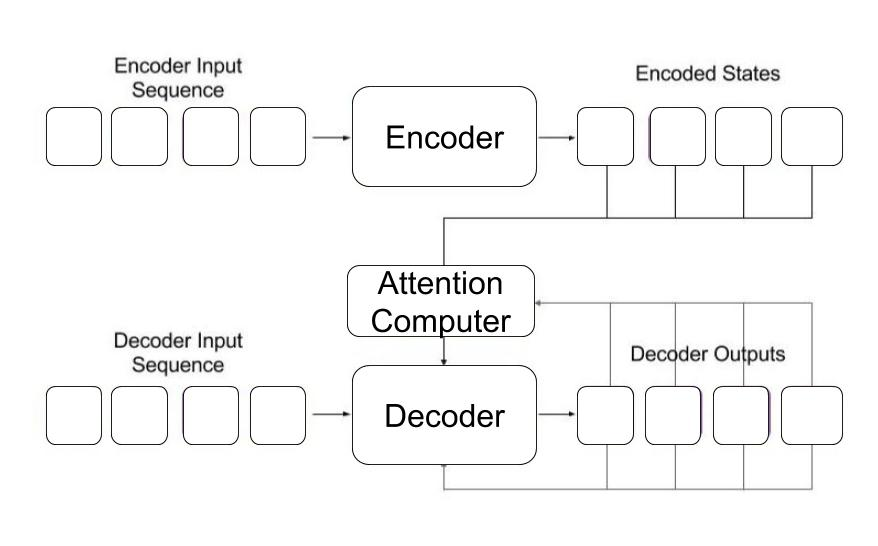
\includegraphics[width=\linewidth]{figures/Attention-Model.jpg}	
				\captionof{figure}{Encoder - Decoder Mechanism with Attention}
				\label{fig: Encoder - Decoder Mechanism with Attention}
				\end{center}

The equations for the encoder-decoder model with attention using RNN as the neural network architecture is as follows:

Encoder: \begin{equation} h_{t} = RNN(h_{t-1}, X_{t}) \end{equation}
		\begin{equation} C_{0} = h_{t}  \end{equation}

Decoder: \begin{equation} e_{jt} = V_{attn} tanh(U * h_{j} + W * C_{t}) \end{equation}	
		 \begin{equation} \alpha_{jt} = softmax(e_{jt})  \end{equation}
		 \begin{equation} S_{t} = \sum_{j=1}^t\alpha_{it} * h_{j}  \end{equation}  
		 \begin{equation} C_{t} = RNN(C_{t-1}, [e(\hat{y}_{t-1}), S_{t}])  \end{equation} 

Where e$_{jt}$ is the importance of j$^{th}$ input for decoding the t$^{th}$ output and $\alpha$$_{jt}$ is the focus probability on j$^{th}$ input with respect to t$^{th}$ output.
	


\section{Overview of Project Report}

Write it at the end.	
	
	\chapter{Linear optimization of Liquidity Risk Management}
	
\setcounter{secnumdepth}{4}

\titleformat{\paragraph}
{\normalfont\normalsize\bfseries}{\theparagraph}{1em}{}
\titlespacing*{\paragraph}
{0pt}{3.25ex plus 1ex minus .2ex}{1.5ex plus .2ex}

\section{Analysis of Saving and Loan Accounts Data}

\section{LPP for Optimization of Assets}

\subsection{Prior Work}

\subsection{Algorithm}

\subsection{Illustration}

\subsection{Computational Complexity}

\subsection{Comparative Analysis}

\subsection{Conclusion }










	
	\chapter{LSTM implementation for Prediction of Stock Price}
	
\setcounter{secnumdepth}{4}

\titleformat{\paragraph}
{\normalfont\normalsize\bfseries}{\theparagraph}{1em}{}
\titlespacing*{\paragraph}
{0pt}{3.25ex plus 1ex minus .2ex}{1.5ex plus .2ex}

%--------------------------------------------------------------------------------
\section{Prior Work}

Prediction of stock prices is the famous problem for several years now. In the era of deep learning various researchers have done the contribution to this topic. Hao Li et al. (2018)\cite{} proposed a Attention based Multi Input LSTM for prediction of opening price given the historical values. It uses attention mechanism for noise filtering and extracting the related information from related stocks. Yao Qin et al. (2017)\cite{} proposed a dual attention based RNN for prediction of treading index using the historical prices of 81 different stocks. The dual attention consists of the input attention mechanism for encoder and a temporal attention mechanism for decoder. Rather et al. (2015)\cite{} proposed the hybrid approach containing RNN and statistical models for prediction of stock price. 

%--------------------------------------------------------------------------------
\section{Algorithm}

The data is collected prior from 2013 to 2018 for the historical stock price of Infosys stock named INFY. The algorithm is trained on the 90\% of the data and tested on the rest of the 10\% of the data. The algorithm is as follows:

\begin{itemize}
		
\item \textbf{Task: } Prediction of Stock Price
			
\item \textbf{Data: } \{X\textsubscript{i} : Open\textsubscript{i}, High\textsubscript{i}, Low\textsubscript{i} ; Y\textsubscript{i} : Close\textsubscript{i} \}$_{i =1}^{N}$		%\textsubscript{i = 1}\textsuperscript{N}
			
\item \textbf{Model: } LSTM: \begin{equation} h_{t}, C_{t} = LSTM(h_{t-1}, C_{t-1}, X_{t}) \end{equation} 	
			
\item \textbf{Parameters: } W$_{f}$, b$_{f}$, W$_{i}$, b$_{i}$, W$_{c}$,  b$_{c}$, W$_{o}$, b$_{o}$ 

\item \textbf{Loss Function: } \begin{equation}Mean Squared Error (MSE) =  \frac{1}{n}\Sigma_{i=1}^{n} (Predicted\_Y_{i} - Y_{i})^2 \end{equation}

\item \textbf{Algorithm: } Adam is the algorithm used for learning the parameters for the LSTM model.


\begin{algorithm}[H]

\caption{Learning Parameters of LSTM for Prediction of Stock Price}

\begin{algorithmic}[1] 
						
\STATE Parameter Initialization: \{strategy = Uniform\} 

\STATE $\emph{epoch} \gets Positive\_Integer$

\STATE \emph{while(eopch > 0)}:

\STATE \tab	Forward Propagation of Data in Model

\STATE \tab	Compute Loss using Loss Function

\STATE \tab	Compute Gradients with respect to Loss

\STATE \tab	Update the Parameters in Backward Propagation	

\STATE\tab	$\emph{epoch} \gets \emph{epoch}-1$

\end{algorithmic}

\end{algorithm}

\end{itemize}

%-----------------------------------------------------------------------------------------------------------------------------
\section{Illustration}
%\paragraph{}
The experimental setup was done in Google Colab, a facility provided by Google Inc. to students and researchers for training deep learning algorithms where they provide free GPU. The computational specification of Colab is as follows:
\begin{itemize}
\item CPU model name: Intel(R) Xeon(R) CPU @ 2.30GHz  
\item No. of Processors : 2
\item CPU Cache Size : 46080 KB
\item GPU Name : Tesla T4
\item GPU Memory : 16 GB (15079MiB usble)
\item RAM : 12.9 GB
\end{itemize}

%\paragraph{}
The programming language used for performing experiment is Python 3.6. The packages used for the experiment include sklearn, keras, math, time, pandas, numpy, pandas\_datareader, matplotlib, h5py,statsmodels, etc.

The hyper-parameters that were fine tuned during the experiment for better performance of the model are as follows with their fine tuned values:

\begin{itemize}

\item seq\_len = 22		\# Input Window Size

\item shape = [4, seq\_len, 1] 	\# No. of Features, Window, Output

\item epochs = 90 		\# No. of times the the forward and backward propagation happens on whole training data through the model

\item dropout rate = 0.3 		\# that percent of neurons from the model will be dropped for each epoch randomly

\item decay = 0.2 		\# parameter decay rate for Adam optimizer

\item neurons = [512, 512, 64, 1]	\# the different combinations of neurons is tried for optimization


\end{itemize}

%\paragraph{}
The architecture of the model used for experimentation is as follows:

%				\begin{center}
%				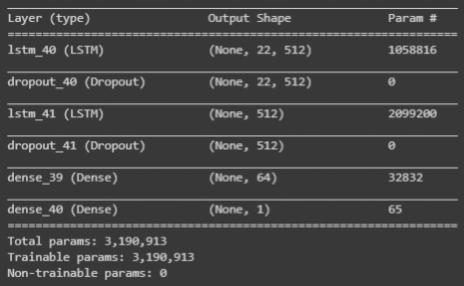
\includegraphics[width=\linewidth]{figures/Model-Sumary.jpg}	
%				\captionof{figure}{The architecture of the LSTM model}
%				\label{fig: The architecture of the LSTM model}
%				\end{center}


\begin{table}[h!]
  \begin{center}
    \caption{The architecture of the LSTM model}
    \label{tab:The architecture of the LSTM model}
    \begin{tabular}{l|l|l} % <-- Alignments: 1st column left, 2nd middle and 3rd right, with vertical lines in between
      \hline
      \textbf{Layer (type)} & \textbf{Output Shape} & \textbf{Param \#}\\
	\hdashline
	\hdashline
      lstm\_40 (LSTM) & (None, 22, 512) & 1058816\\
	\hline
      dropout\_40 (Dropout) &  (None, 22, 512) & 0\\
	\hline
      lstm\_41 (LSTM) & (None, 512) & 2099200 \\
	\hline
      dropout\_41 (Dropout) & (None, 512) & 0 \\
	\hline
      dense\_39 (Dense) & (None, 64) & 32832 \\
	\hline
      dense\_40 (Dense) & (None, 1) & 65 \\
	\hdashline
	\hdashline
	\multicolumn{3}{l}{Total params: 3,190,913} \\
	\multicolumn{3}{l}{Trainable params: 3,190,913} \\
	\multicolumn{3}{l}{Non-trainable params: 0} \\
	\hline
    \end{tabular}
  \end{center}
\end{table}


%\end{itemize}
				\begin{center}
				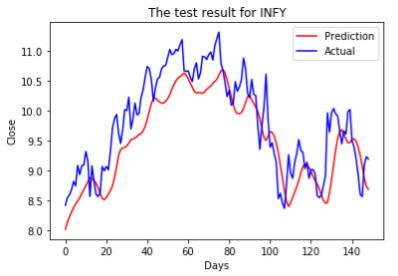
\includegraphics[width=\linewidth]{figures/test-data-results.jpg}	
				\captionof{figure}{Plot showing of Actual and Predicted values}
				\label{fig: Plot showing of Actual and Predicted values}
				\end{center}

%--------------------------------------------------------------------------------
\section{Computational Complexity}

Computational complexity of LSTM is O(Z),\\
  where Z = 4 * \#IP * h + 4 * h$^{2}$ + 3 * h + h * \#OP , \\
 \tab\#IP: Number of inputs\\
 \tab\#h: Number of hidden layers\\
 \tab\#OP: Number of outputs\\

The total time taken by the model to train is 1min 9 sec.
%--------------------------------------------------------------------------------
\section{Comparative Analysis} 

After training the LSTM model we have tested the model on unseen test data and the MSE is as follows:
\begin{itemize}
\item MSE on Train Data: 0.00128 MSE
\item MSE on Test Data: 0.00230 MSE

The predictions of ARIMA and Auto-ARIMA models were taken into consideration for comparison with predictions of LSTM model. 
\begin{itemize}
\item MSE on Test Data of ARIMA Model:  0.576 MSE
\item MSE on Test Data of Auto-ARIMA Model:  0.695 MSE
\end{itemize}
				\begin{center}
				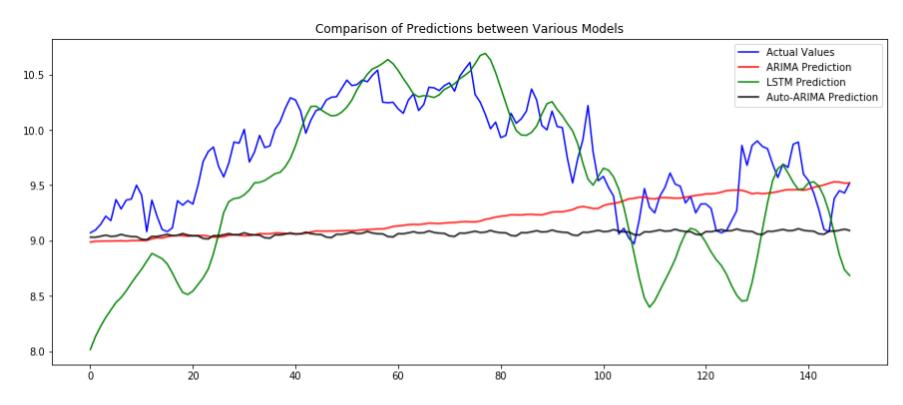
\includegraphics[width=\linewidth]{figures/Comp-ARIMA-LSTM.jpg}	
				\captionof{figure}{Comparison of Prediction between ARIMA Model and LSTM Model with Actual Values}
				\label{fig: Comparison of Prediction between ARIMA Model and LSTM Model with Actual Values}
				\end{center}
\end{itemize}
%--------------------------------------------------------------------------------
\section{Conclusion }

In this chapter we have discussed about the model architecture, its parameters, and tuning the parameters for optimization of performance of the model. The LSTM model performed far better than the statistical models.

	
	\chapter{Conclusion}
	
\setcounter{secnumdepth}{4}

\titleformat{\paragraph}
{\normalfont\normalsize\bfseries}{\theparagraph}{1em}{}
\titlespacing*{\paragraph}
{0pt}{3.25ex plus 1ex minus .2ex}{1.5ex plus .2ex}

%--------------------------------------------------------------------------------
\section{Prior Work}

Prediction of stock prices is the famous problem for several years now. In the era of deep learning various researchers have made the contributions to this topic. Hao Li et al. (2018)\cite{} proposed a Attention based Multi Input LSTM for prediction of opening price given the historical values. It uses attention mechanism for noise filtering and extracting the related information from related stocks. Yao Qin et al. (2017)\cite{} proposed a dual attention based RNN for prediction of treading index using the historical prices of 81 different stocks. The dual attention consists of the input attention mechanism for encoder and a temporal attention mechanism for decoder. Rather et al. (2015)\cite{} proposed the hybrid approach containing RNN and statistical models for prediction of stock price. 

%--------------------------------------------------------------------------------
\section{Algorithm}

The data is collected prior from 2013 to 2018 for the historical stock price of Infosys stock named INFY. The algorithm is trained on the 90\% of the data and tested on the rest of the 10\% of the data. The algorithm is as follows:

\begin{itemize}
		
\item \textbf{Task: } Prediction of Stock Price
			
\item \textbf{Data: } \{X\textsubscript{i} : Open\textsubscript{i}, High\textsubscript{i}, Low\textsubscript{i} ; Y\textsubscript{i} : Close\textsubscript{i} \}$_{i =1}^{N}$		%\textsubscript{i = 1}\textsuperscript{N}
			
\item \textbf{Model: } LSTM: \begin{equation} h_{t}, C_{t} = LSTM(h_{t-1}, C_{t-1}, X_{t}) \end{equation} 	
			
\item \textbf{Parameters: } W$_{f}$, b$_{f}$, W$_{i}$, b$_{i}$, W$_{c}$,  b$_{c}$, W$_{o}$, b$_{o}$ 

\item \textbf{Loss Function: } \begin{equation}Mean Squared Error (MSE) =  \frac{1}{n}\Sigma_{i=1}^{n} (Predicted\_Y_{i} - Y_{i})^2 \end{equation}

\item \textbf{Algorithm: } Adam is the algorithm used for learning the parameters for the LSTM model.


\begin{algorithm}[H]

\caption{Learning Parameters of LSTM for Prediction of Stock Price}

\begin{algorithmic}[1] 
						
\STATE Parameter Initialization: \{strategy = Uniform\} 

\STATE $\emph{epoch} \gets Positive\_Integer$

\STATE \emph{while(eopch > 0)}:

\STATE \tab	Forward Propagation of Data in Model

\STATE \tab	Compute Loss using Loss Function

\STATE \tab	Compute Gradients with respect to Loss

\STATE \tab	Update the Parameters in Backward Propagation	

\STATE\tab	$\emph{epoch} \gets \emph{epoch}-1$

\end{algorithmic}

\end{algorithm}

\end{itemize}

%-----------------------------------------------------------------------------------------------------------------------------
\section{Illustration}
%\paragraph{}
The experimental setup was done in Google Colab, a facility provided by Google Inc. to students and researchers for training deep learning algorithms where they provide free GPU. The computational specification of Colab is as follows:
\begin{itemize}
\item CPU model name: Intel(R) Xeon(R) CPU @ 2.30GHz  
\item No. of Processors : 2
\item CPU Cache Size : 46080 KB
\item GPU Name : Tesla T4
\item GPU Memory : 16 GB (15079MiB usble)
\item RAM : 12.9 GB
\end{itemize}

%\paragraph{}
The programming language used for performing experiment is Python 3.6. The packages used for the experiment include sklearn, keras, math, time, pandas, numpy, pandas\_datareader, matplotlib, h5py,statsmodels, etc.

The hyper-parameters that were fine tuned during the experiment for better performance of the model are as follows with their fine tuned values:

\begin{itemize}

\item seq\_len = 22		\# Input Window Size

\item shape = [4, seq\_len, 1] 	\# No. of Features, Window, Output

\item epochs = 90 		\# No. of times the the forward and backward propagation happens on whole training data through the model

\item dropout rate = 0.3 		\# that percent of neurons from the model will be dropped for each epoch randomly

\item decay = 0.2 		\# parameter decay rate for Adam optimizer

\item neurons = [512, 512, 64, 1]	\# the different combinations of neurons is tried for optimization


\end{itemize}

%\paragraph{}
The architecture of the model used for experimentation is as follows:

				\begin{center}
				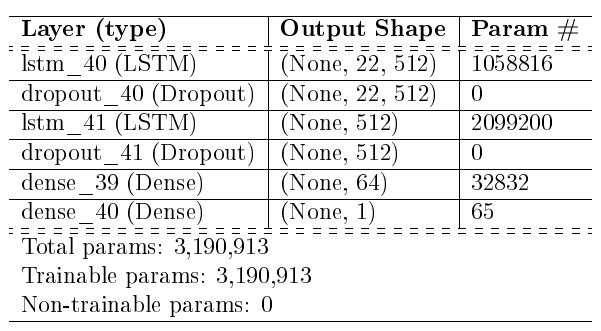
\includegraphics[width=\linewidth]{figures/architecture-of-LSTM.jpg}	%Model-Sumary
				\captionof{figure}{The architecture of the LSTM model}
				\label{fig: The architecture of the LSTM model}
				\end{center}


%architecture-of-LSTM



%\begin{table}[h!]
%  \begin{center}
%    \caption{The architecture of the LSTM model}
%    \label{tab:The architecture of the LSTM model}
%    \begin{tabular}{l|l|l} % <-- Alignments: 1st column left, 2nd middle and 3rd right, with vertical lines in between
%      \hline
%      \textbf{Layer (type)} & \textbf{Output Shape} & \textbf{Param \#}\\
%	\hdashline
%	\hdashline
%      lstm\_40 (LSTM) & (None, 22, 512) & 1058816\\
%	\hline
%      dropout\_40 (Dropout) &  (None, 22, 512) & 0\\
%	\hline
%      lstm\_41 (LSTM) & (None, 512) & 2099200 \\
%	\hline
%      dropout\_41 (Dropout) & (None, 512) & 0 \\
%	\hline
%      dense\_39 (Dense) & (None, 64) & 32832 \\
%	\hline
%      dense\_40 (Dense) & (None, 1) & 65 \\
%	\hdashline
%	\hdashline
%	\multicolumn{3}{l}{Total params: 3,190,913} \\
%	\multicolumn{3}{l}{Trainable params: 3,190,913} \\
%	\multicolumn{3}{l}{Non-trainable params: 0} \\
%	\hline
%    \end{tabular}
%  \end{center}
%\end{table}

\section{Results}


%\end{itemize}
				\begin{center}
				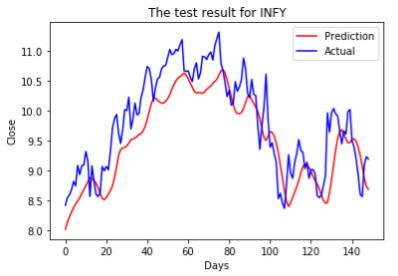
\includegraphics[width=\linewidth]{figures/test-data-results.jpg}	
				\captionof{figure}{Plot showing of Actual and Predicted values}
				\label{fig: Plot showing of Actual and Predicted values}
				\end{center}

%--------------------------------------------------------------------------------
\section{Computational Complexity}

Computational complexity of LSTM is O(Z),\\
  where Z = 4 * \#IP * h + 4 * h$^{2}$ + 3 * h + h * \#OP , \\
 \tab\#IP: Number of inputs\\
 \tab\#h: Number of hidden layers\\
 \tab\#OP: Number of outputs\\

The total time taken by the model to train is 1min 9 sec.
%--------------------------------------------------------------------------------
\section{Comparative Analysis} 

After training the LSTM model we have tested the model on unseen test data and the MSE is as follows:
\begin{itemize}
\item MSE on Train Data: 0.00128 MSE
\item MSE on Test Data: 0.00230 MSE

The predictions of ARIMA and Auto-ARIMA models were taken into consideration for comparison with predictions of LSTM model. 
\begin{itemize}
\item MSE on Test Data of ARIMA Model:  0.576 MSE
\item MSE on Test Data of Auto-ARIMA Model:  0.695 MSE
\end{itemize}
				\begin{center}
				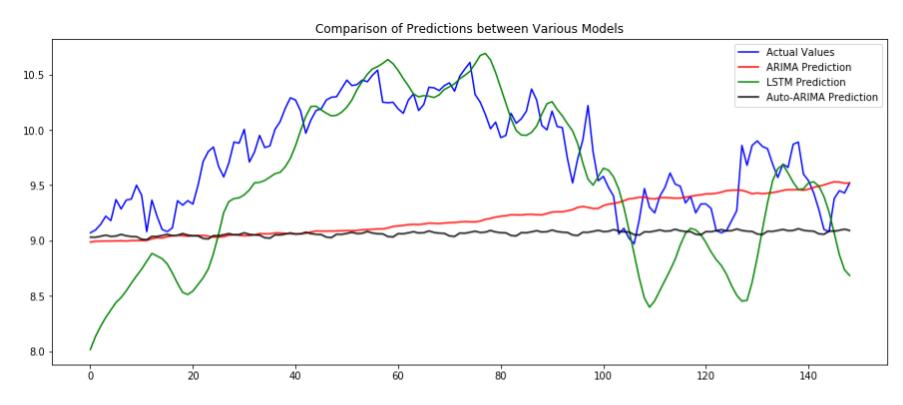
\includegraphics[width=\linewidth]{figures/Comp-ARIMA-LSTM.jpg}	
				\captionof{figure}{Comparison of Prediction between ARIMA, Auto-ARIMAl and LSTM Model with Actual Values}
				\label{fig: Comparison of Prediction between ARIMA, Auto-ARIMAl  and LSTM Model with Actual Values}
				\end{center}
\end{itemize}
%--------------------------------------------------------------------------------
\section{Conclusion }

In this chapter we have discussed about the model architecture, its parameters, and tuning the parameters for optimization of performance of the model. The LSTM model performed far better than the statistical models.

	
	\chapter{Future Work}
	
\setcounter{secnumdepth}{4}

\titleformat{\paragraph}
{\normalfont\normalsize\bfseries}{\theparagraph}{1em}{}
\titlespacing*{\paragraph}
{0pt}{3.25ex plus 1ex minus .2ex}{1.5ex plus .2ex}


The work done in this thesis tries to solve ALM problem for bank. The second chapter simulates the ALM environment of the bank and gives the brief understanding of the concept. 
It also gives nice insights from the data which can be utilized for maximizing profit.\\

The third chapter discusses the single objective optimization method for liquidity risk management using Linear Programming Formulation using objective function as maximizing the profit of the bank.\\

The third chapter makes an attempt to predict the stock price of the particular stock based on it's historical values using the novelty of the deep learning techniques. The LSTM model trained on the data completely outperforms the traditional statistical models.
	
	%\clearpage
	%\addcontentsline{toc}{chapter}{Bibliography}
	%\begin{thebibliography}{1}
		\bibliographystyle{ieeetr} 
		\footnotesize
		
		\bibitem{1}
		Teng, Fan, and Qingwei Zhang. "Empirical Analysis on Interest-Rate Risk to Chinese Life Insurers and Scenario Testing." In 2011 International Conference on Management and Service Science, pp. 1\-3. IEEE, 2011.

		
		\bibitem{2}
		Vaswani, Ashish, Noam Shazeer, Niki Parmar, Jakob Uszkoreit, Llion Jones, Aidan N. Gomez, Łukasz Kaiser, and Illia Polosukhin. "Attention is all you need." In Advances in neural information processing systems, pp. 5998\-6008. 2017.

		
		\bibitem{3}
		 Gülpinar, Nalan, and Dessislava Pachamanova. "A robust optimization approach to asset-liability management under time-varying investment opportunities." Journal of Banking \& Finance 37, no. 6 (2013): 2031\-2041.
		
		\bibitem{4}
		Li, Hongxi, and Guotai Chi. "Assets and Liabilities Portfolio Optimal Model based on ES Controlled Interest Rate Risk." In Proceedings of the International Conference on Business and Information Management, pp. 1\-5. ACM, 2017.
		
		
		\bibitem{5} 
		Images are drawn in a software package called \emph{Jupyter Notebook}.
		
		\bibitem{6}
		 Qin, Yao, Dongjin Song, Haifeng Chen, Wei Cheng, Guofei Jiang, and Garrison Cottrell. "A dual-stage attention-based recurrent neural network for time series prediction." arXiv preprint arXiv:1704.02971 (2017).
		
		\bibitem{7}
		 Liu, Jian, Yubo Chen, Kang Liu, and Jun Zhao. "Attention-Based Event Relevance Model for Stock Price Movement Prediction." In China Conference on Knowledge Graph and Semantic Computing, pp. 37\-49. Springer, Singapore, 2017.
		  
		 \bibitem{8}
		 Li, Hao, Yanyan Shen, and Yanmin Zhu. "Stock Price Prediction Using Attention-based Multi-Input LSTM." In Asian Conference on Machine Learning, pp. 454\-469. 2018.

		\bibitem{9}
		Liu, Huicheng. "Leveraging Financial News for Stock Trend Prediction with Attention-Based Recurrent Neural Network." arXiv preprint arXiv:1811.06173 (2018).
		
		\bibitem{10}
		 B. Yan and S. Gregory, Detecting community structure in networks using edge prediction methods, \{Journal of Statistical and Mechanical\}, P09008 (2012).
		 
		 \bibitem{11}
		  https://www.rbi.org.in/scripts/NotificationUser.aspx?Id=16\&Mode=0
		 
		 \bibitem{12}
		 Images are drawn in a software package called \emph{RStudio} and \emph{Jupyter Notebook}.		 
		 
		 \bibitem{12}
		 Goodfellow, Ian, Yoshua Bengio, and Aaron Courville. Deep learning. MIT press, 2016.
		 
		 \bibitem{14}		 
		 \url{http://www.rstudio.com/}		 
		 
		 \bibitem{15}
		 \url{http://en.wikipedia.org/wiki/Deep\_learning}		 
		 
		 \bibitem{16}
		 Mounika, P.; Sastry, V.N. (2011). “Cash-flow optimization models for asset liability management” (M-tech project report, IDRBT) 

		 
		 \bibitem{17}
		 Chaudhury, Rahul; Sastry, V.N. (2014). “Fuzzy optimization based asset liability management” (M-Tech project report, IDRBT) 

		 
		 \bibitem{18}
		 Shumway, Robert H., and David S. Stoffer. Time series analysis and its applications: with R examples. Springer, 2017.	
		 
		 \bibitem{19}
		 https://data.world/lpetrocelli/czech-financial-dataset-real-anonymized-transactions/workspace/data-dictionary
		 
		 
		
\end{thebibliography}

	
\end{document}
